\subsection{Outsider detection}
\label{outsider_detection}
We built 61*60/2 = 1830 bootstrapped regresson models to analyse a total of
296639 distinct PPS. A total of 67\% of the trained regression models passed
model quality control. Let us use the \textit{Drosophila
simulans}/\textit{Wolbachia} pair as an example of what was done. Figure
~\ref{fig:pca_analysis} shows a principal component analysis (PCA)
visualization of sequence clustering based on the normalized values of bit
scores for the \textit{Drosophila simulans} and \textit{Wolbachia} metagenomic
experiment. A clear separation of sequences can be observed even without the
use of regression analysis by PCA alone; however, we used PCA analysis only for
illustrative purposes.
\begin{center}
\begin{figure}
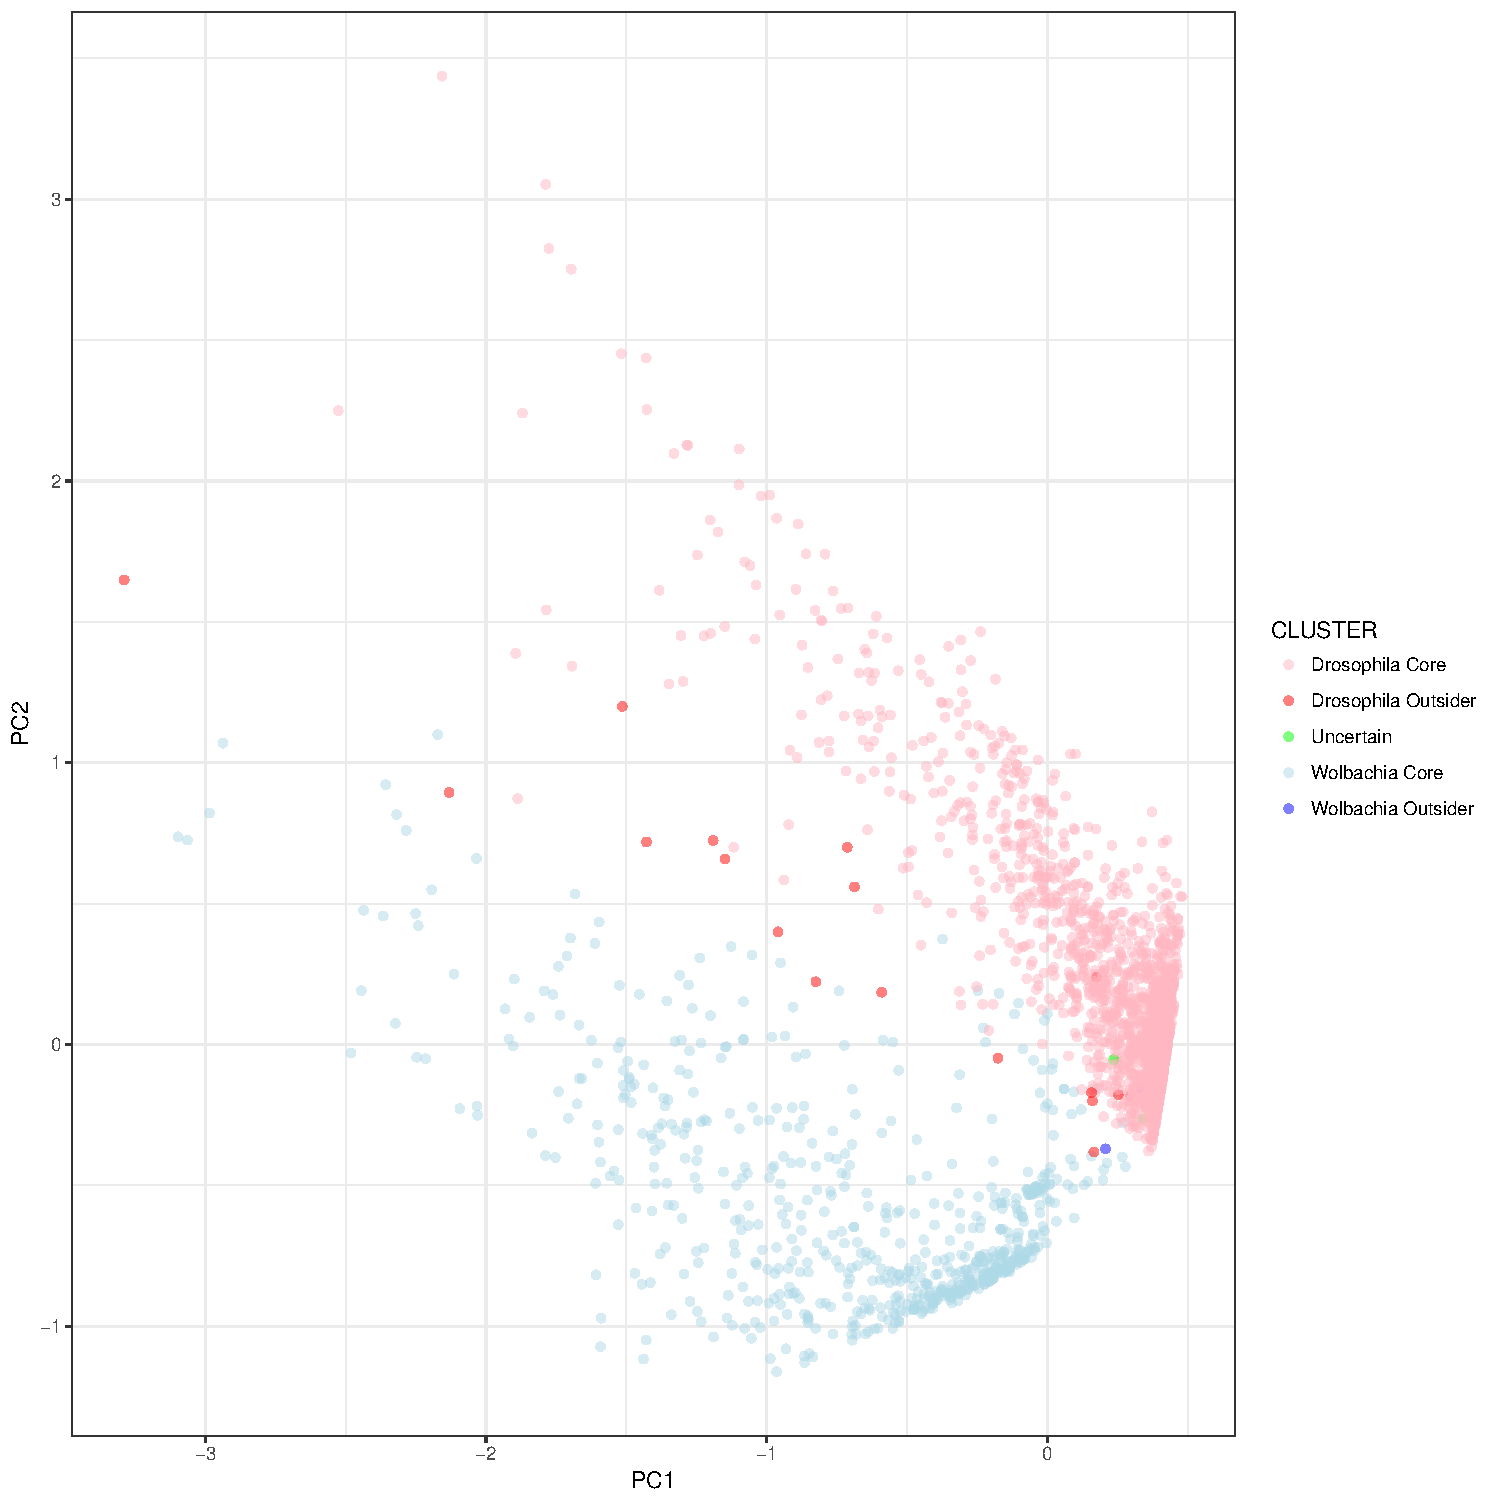
\includegraphics[width=12cm]{figures/w_eds_vs_ds_bootstrapped_pc1_pc2.pdf}
\caption{PCA analysis for clusters of predicted \textit{Drosophila simulans}
	and \textit{Wolbachia PPS}.}
\label{fig:pca_analysis}
\end{figure}
\end{center}
Figure ~\ref{fig:rsquared_barplot} contains an overview of the regression
models for \textit{Drosophila simulans} and each genome it was compared with.
Core genes are PPS from a genome that were correctly assigned to that
particular genome by the regression analysis. Outsider PPS are sequences that were
assigned to the other genome. The uncertain PPS are marked grey.
\begin{center}
\begin{figure}
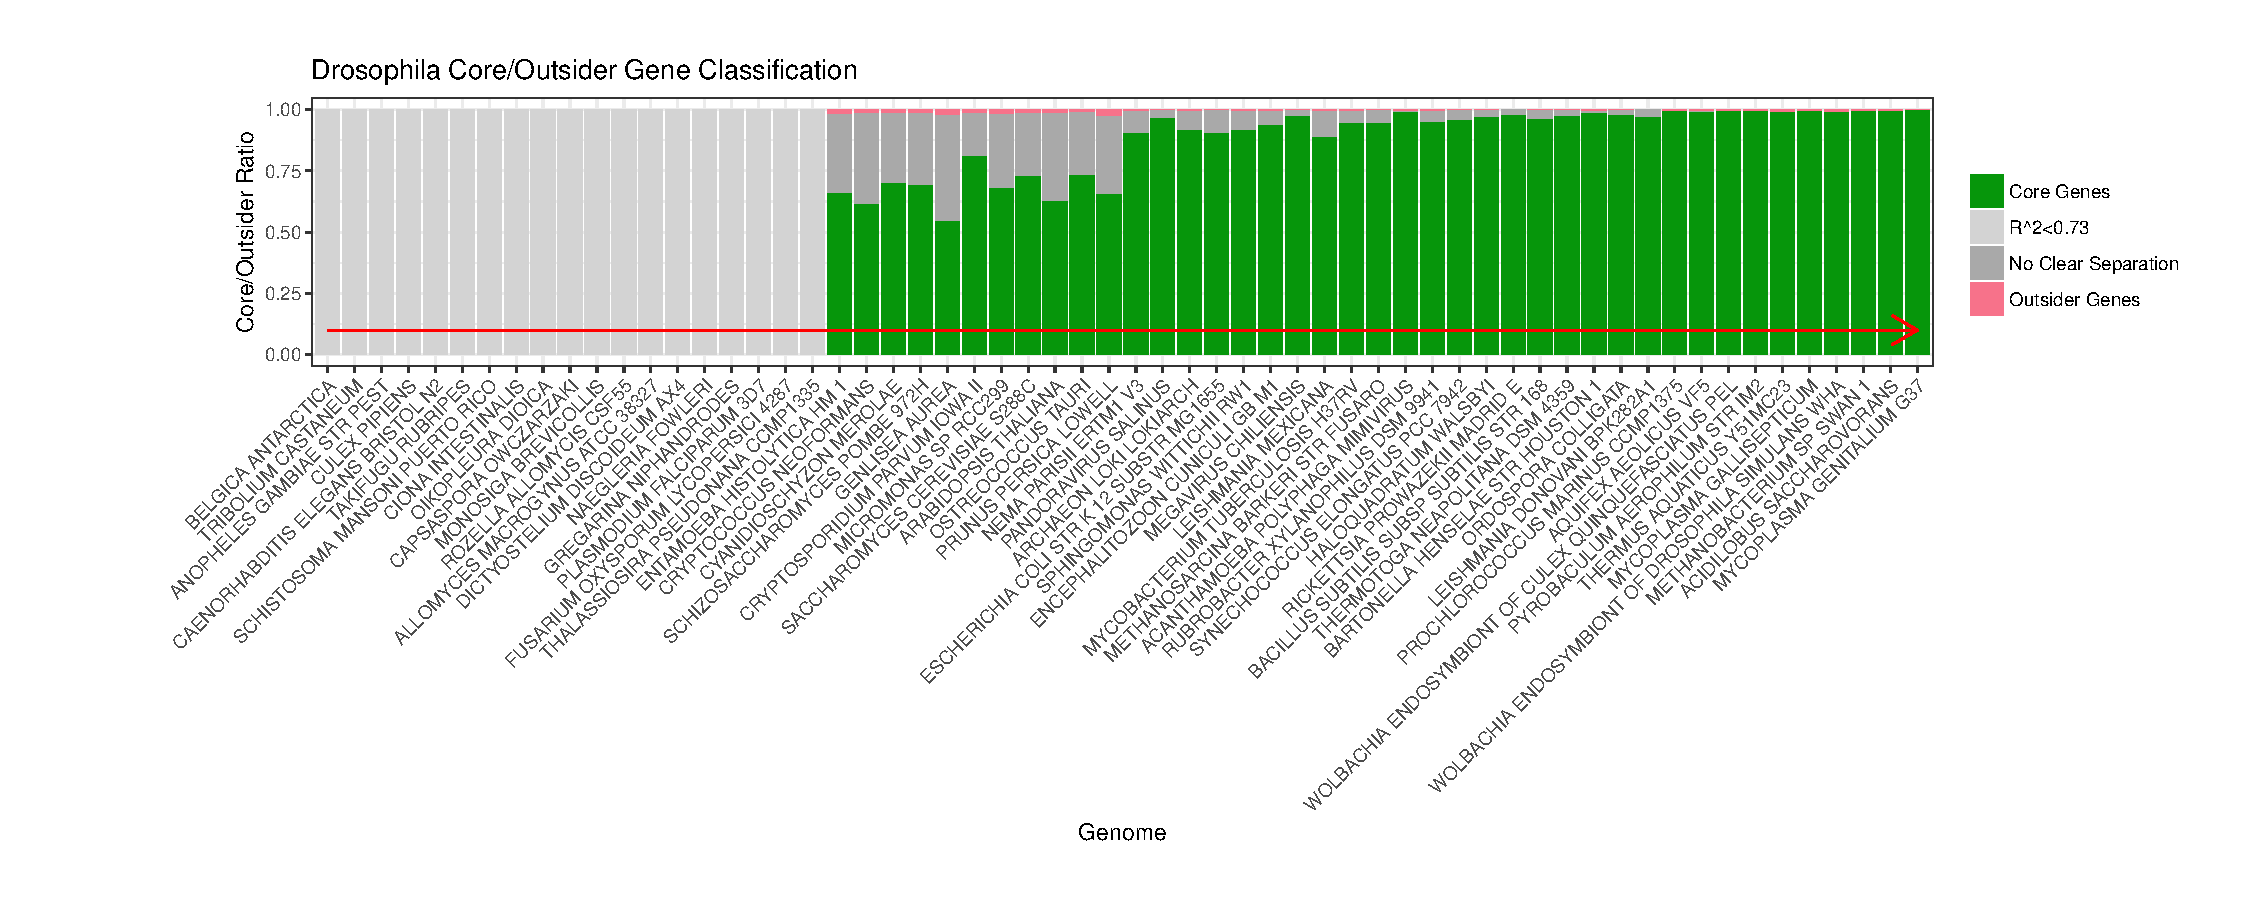
\includegraphics[width=12cm]{figures/core_outsider_barplot_bootstrapped.pdf}
\caption{The fraction of core/outsider \textit{Drosophila simulans} genes in
each model. The gray coloring represents the genome pairs where separation of genes was not successful (R2 <
0.73)}
\label{fig:rsquared_barplot}
\end{figure}
\end{center}

Figure ~\ref{fig:rsquared_curve} presents the $R^2$ values obtained for
regression models using \textit{Drosophila simulans} and each other genome in
our dataset (higher $R^2$ values are better). As expected, it is difficult to
separate the sequences of closely related arthropods (low $R^2$ values) but
it is easy to fulfill this task for distantly related genome pairs such as
\textit{Drosophila} and \textit{Mycoplasma}.
\begin{center}
\begin{figure}
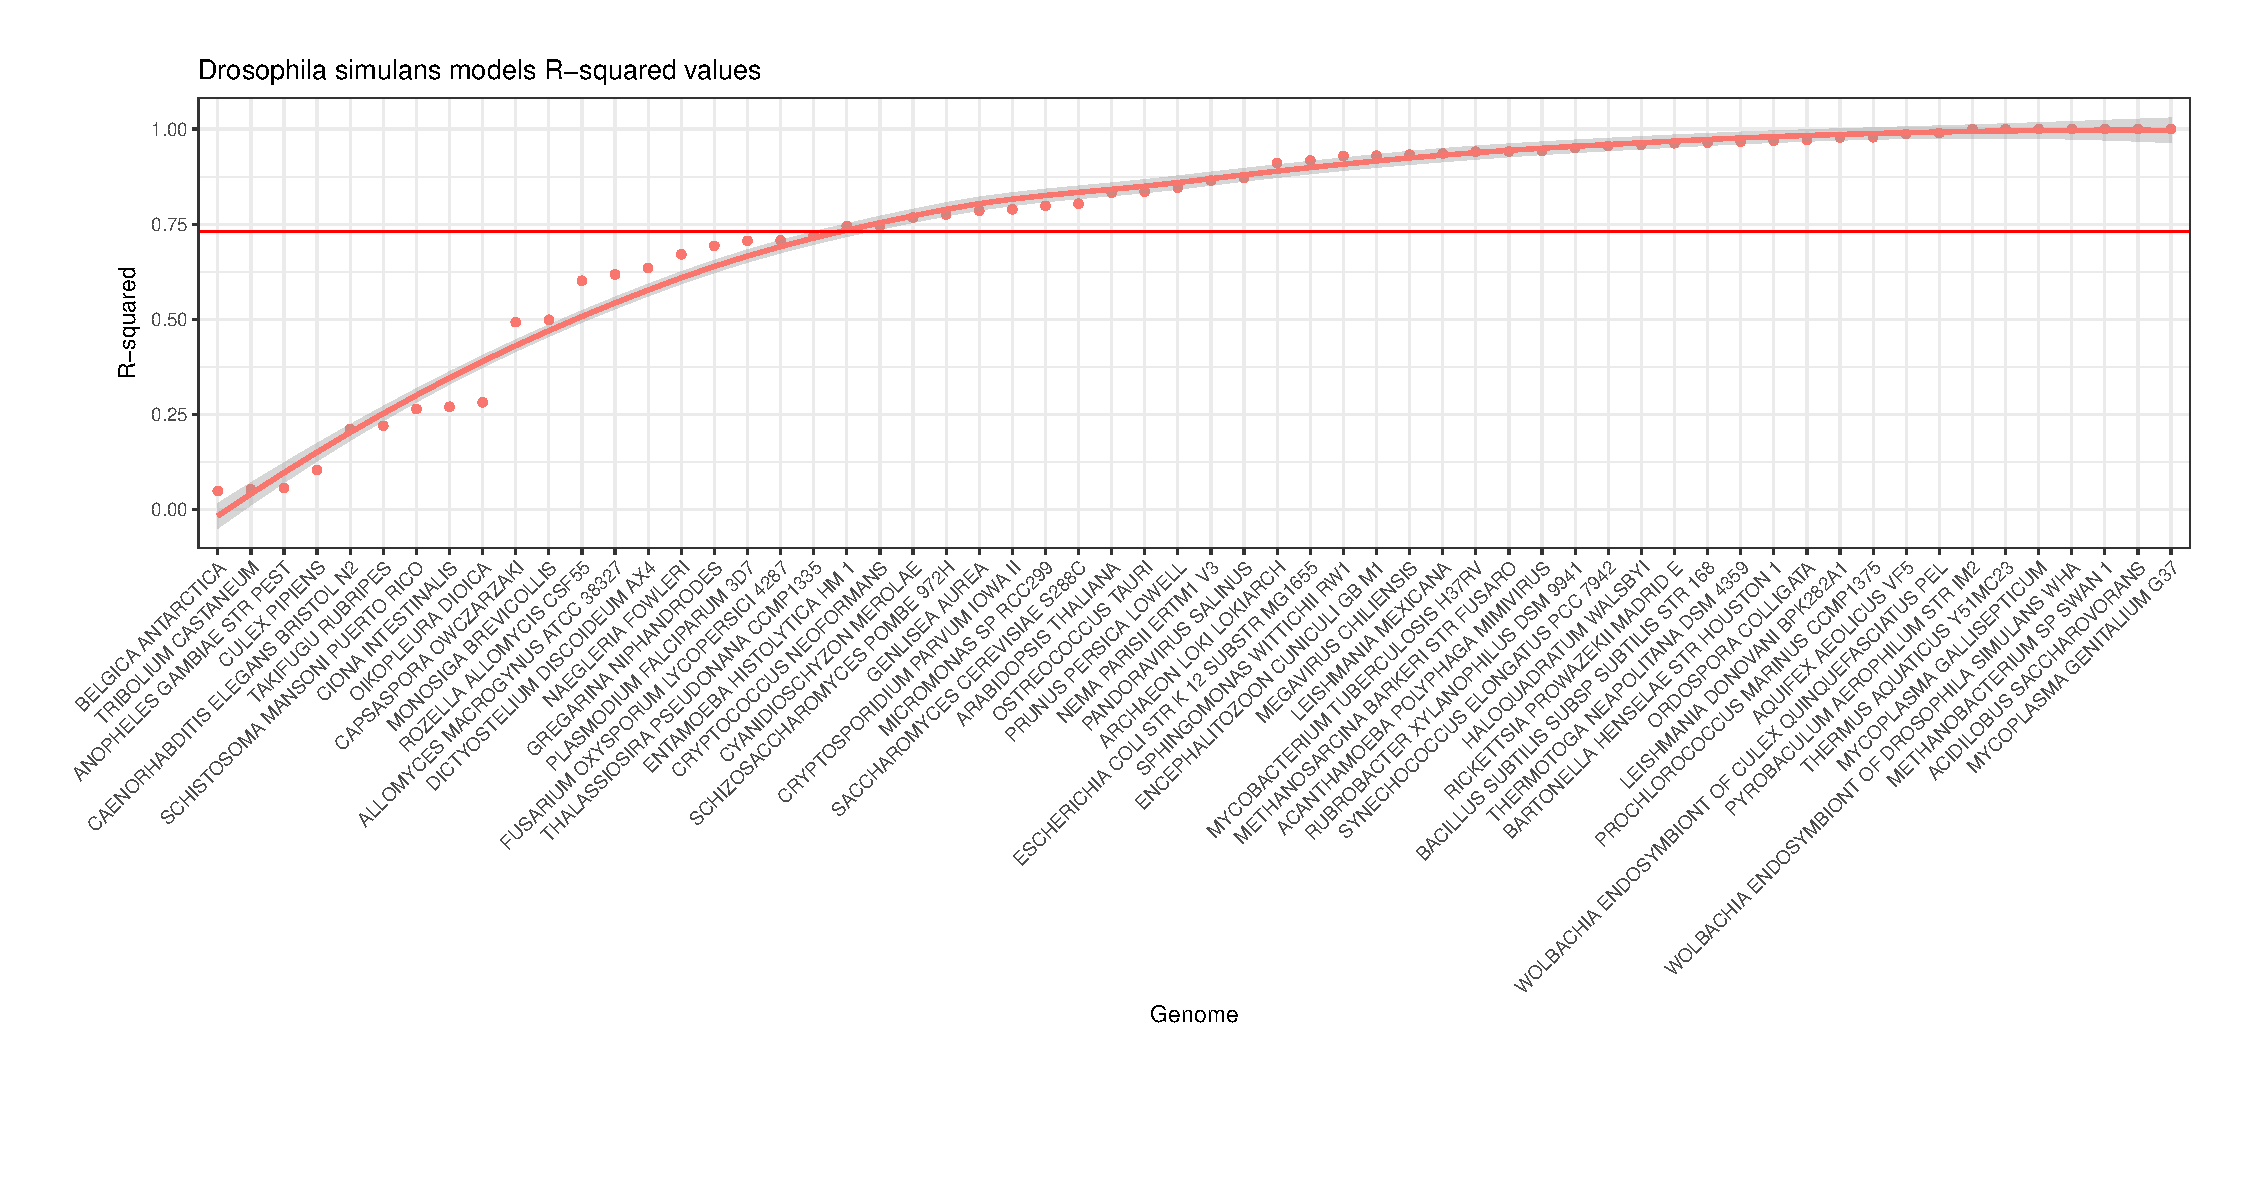
\includegraphics[width=12cm]{figures/rsq_drosoph_bootstrapped.pdf}
\caption{$R^2$ values for regression models for \textit{Drosophila} vs. all
other genomes.}
\label{fig:rsquared_curve}
\end{figure}
\end{center}
The majority of sequences (287942, 97.1\%) from each analyzed genome were
classified as core sequences in all metagenomic experiment with validated
regression models. 3992 (1.3\%) PPS were classified as "outsider" by one model
(in one comparison of two genomes). The remaining 4705 (1.6\%) sequences were
classified as “outsider multiple” and are the most likely candidates for HGT.
The list of protein-coding open reading frames classified as “outsider once”,
or “outsider multiple” along with their FASTA sequences is available for
download: [link]. For the fraction of “outsider once” and “outsider multiple”
genes varies from genome to genome see Supplement. An important limitation is
that our approach does not distinguish HGT from genomic contaminations. Thus
the observed differences in Core/Outsider ratio between different genomes, does
not necessarily indicate that some genomes are more prone to the acquisition of
sequences due to HGT. We used a PFAM analysis to check for any PFAM domains are
significantly overrepresented PPS that were classified as outsiders by some of
the models. A list of top-ranked findings (ranked by significance) is presented
in Table ~\ref{table:pfam_domains}. We would like to highlight some of the most
interesting findings.
\begin{center}
\begin{table}
{
\setstrech{1.0}
\pgfplotstabletypeset[
    col sep=comma,
    string type,
    every head row/.style={%
        before row={\hline
            \multicolumn{2}{c}{Overrepresented PFAM Domains} & \\
        },
        after row=\hline
    },
    every last row/.style={after row=\hline},
    columns/pdom/.style={column name=PFAM Domain, column type=l},
    columns/spec/.style={column name=Species, column type=l},
    columns/pval/.style={column name=P-value, column type=c}
    ]{resources/pfam_domain_table.csv}
\caption{PFAM domains that are overrepresented among predicted horizontally
transferred protein-coding sequences}
\label{table:pfam_domains}
}
\end{table}
\end{center}
